\documentclass{article}

% Language setting
% Replace `english' with e.g. `spanish' to change the document language
\usepackage{polski}
\usepackage[utf8]{inputenc}

% Set page size and margins
% Replace `letterpaper' with `a4paper' for UK/EU standard size
\usepackage[letterpaper,top=2cm,bottom=2cm,left=3cm,right=3cm,marginparwidth=1.75cm]{geometry}

% Useful packages
\usepackage{amsmath}
\usepackage{graphicx}
\usepackage[colorlinks=true, allcolors=blue]{hyperref}

\title{Praca inżynierska}
\author{Mikołaj Kuszowski}

\begin{document}
\maketitle

\begin{abstract}
      Next sections: 1. TDD - Test-driven development  2. CQRS
\end{abstract}

\section{Spotkanie z biznesem}
      Pierwszym etapem stworzenia aplikacji jest konfrontacja IT z Biznesem. W naszym wypadku Biznesem mogą być klienci czyli zewnętrzne firmy lub inne działy wewnątrz firmy. Biznes przychodzi z problemem, przedstawia swoje cele i wymagania. Dział IT musi więc dobrze rozumieć cele i potrzeby biznesowe, natomiast biznes musi wiedzieć, czy organizacja dysponuje zasobami niezbędnymi do ich realizacji.[https://cyfrowa.rp.pl/technologie/art40278241-konieczna-wspolpraca-miedzy-it-i-biznesem] Łącznikiem między Binzesem, a IT jest analityk biznesowy, który ma wiedzę techniczną oraz jest w stanie w przejrzysty sposób zrozumieć wymagania biznesu.

      Proces wytwarzania oprogramowania możemy rozpocząć od warsztatu o fachowej nazwie "Event Storming". Jest to proces na styku biznesu i produkcji oprogramowania. Takie spotkanie ma na celu przedstawienie przez bisnes jak działa albo jak ma działać domena. Do domeny nie zalicza się tylko aplikacja, ale też ludzie wykonujący jakiś proces czy inne zewnętrzne aplikacje. Dzięki poznaniu domemy można poznać wszystkie procesy występujące docelowo wokół naszej aplikacji co ułatwia zrozumienie całego procesu. Finalnie tylko fragment z przedstawionego podczas event stormingu procesu będzie należał do wytwarzanej aplikacji. Zaletą Event Stormingu jest również lepsze zrozumienie domeny przez biznes, który wcześniej mógł nie być świadomy, że oczywiste według nich procesy mogą być bardziej skomplikowane co mogłoby utrudnić pracę programistyczne. W event stormingu najważniejsze jest poznanie całości domeny, dlatego ważne jest, aby osoby biznesowe przedstawiły wszystkie swoje zadania. Zasadność tych zadań będzie dyskutowana w dalszej części. Podczas takiego spotkania uczestniczą:
      \begin{itemize}
            \item Eksperci domenowi - od strony biznesu
            \item Eksperci techniczni - np. analitycy biznesowi
      \end{itemize}

      Sama forma warsztatu wydaje się dość prosta – do dyspozycji mamy dużą tablicę czy ścianę oraz mnóstwo różnokolorowych karteczek. Każdy z uczestników identyfikuje zdarzenia („Domain Events”), które występują w trakcie działania programu – np. „Utworzono konto użytkownika”, „Zamówiono towar”, czy „Wygenerowano fakturę”. Zdarzenia te zapisuje się na karteczkach i umieszcza na tablicy. [https://bulldogjob.pl/readme/event-storming-pierwszy-krok-do-ddd]. Celem takiego spotkania jest klarowne poznanie domeny (biznesu) i zrozumienie potrzeb oraz wymagań. 

      Wytwarzanie aplikacji zaczniemy od procesu Event Storimngu. Aby ją lepiej zrozumień zdefiniujmy co oznaczają poszczególne kolory karteczek.
      \begin{itemize}
            \item Żółty: Aktor (ang. Actor) - Admin, Klient, Sprzedawca
            \item Niebieski: Polecenie (ang. command) - planujemy coś zmienić
            \item Zielony: Model odczytu (ang. read model) - dane, które wykonują decyzję (np. dane z formularza)
            \item Fioletowy: 
            \item Złoty: Zdarzenia domenowe (ang. domain event) - polecenie zakończone z sukcesem
      \end{itemize}
      Karteczki opcjonalne
      \begin{itemize}
            \item Różowy: Problemy (ang. Issues)
      \end{itemize}

      Event Storming możemy zacząć od procesu zwanego "Big Picture". Proces ten rozpoczynamy od zdefiniowania zdarzeń czyli pomarańczowych karteczek. Aby zdarzenie było prawidłowe musi spełniać następujące wymagania:
      \begin{itemize}
            \item musi być opisane w czasie przeszłym
            \item opisuje zmianę w systemie
            \item występuje w konkretnym momencie w czasie
      \end{itemize}
      W początkowym etapie definiowania zdarzeń nie jest dla nas istotne miejsce ich występowania na osi czasu. Faza definiowania zdarzeń bez ich umieszczania na osi czasu nazywa się chaotyczną eksploracją. Oto początkowo zdefioniowane zdarzenia:
      \begin{figure}[h]
            \centering
            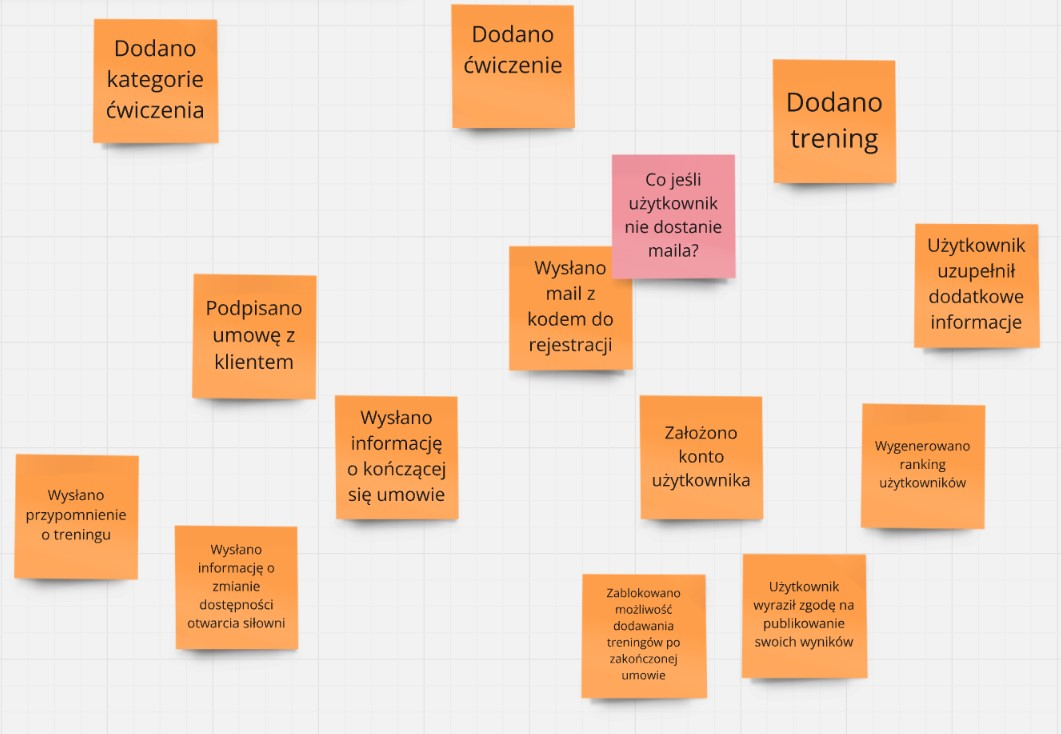
\includegraphics[width=0.9\linewidth]{bigPicture1.jpg}
            \caption{Chaotyczna eksploracja}
      \end{figure}
      Po zdefiniowaniu zdarzeń można poukładać je na osi czasu. Zdarzenia mogące występować w tym samym czasie znajdują się na jednym poziomie (w tej samej kolumnie). Podczas porządkowania zdarzeń na osi czasu mogą pojawić się nowe zdarzenia. Możemy dodawać tutaj również nasze problemy/pytania związane z danym zdarzeniem. Możemy dodać złotą taśmę z nazwą procesu dotyczącą kilku zdarzeń. Jeżeli zdarzenie jest zbyt ogólne powinniśmy je rozbić na kilka mniejszych zdarzeń.
      \begin{figure}[h]
            \centering
            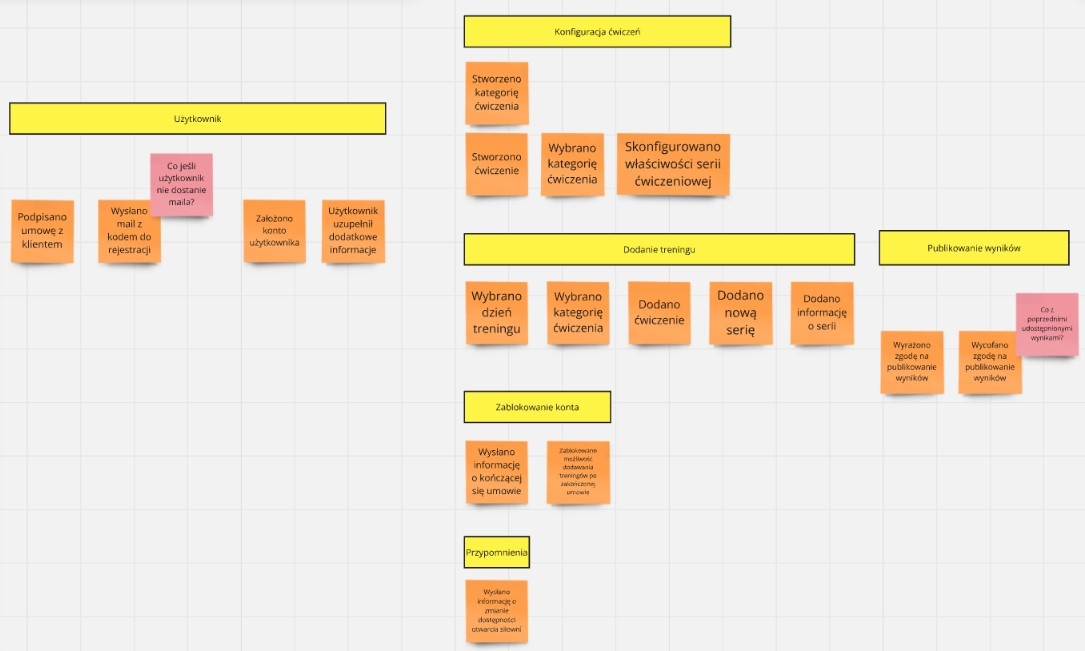
\includegraphics[width=0.9\linewidth]{bigPicture3.jpg}
            \caption{Porządkowanie linii czasu}
      \end{figure}
      Po etapie big picture możemy zacząć fazę zwaną "Process level". 
      \begin{figure}[h]
            \centering
            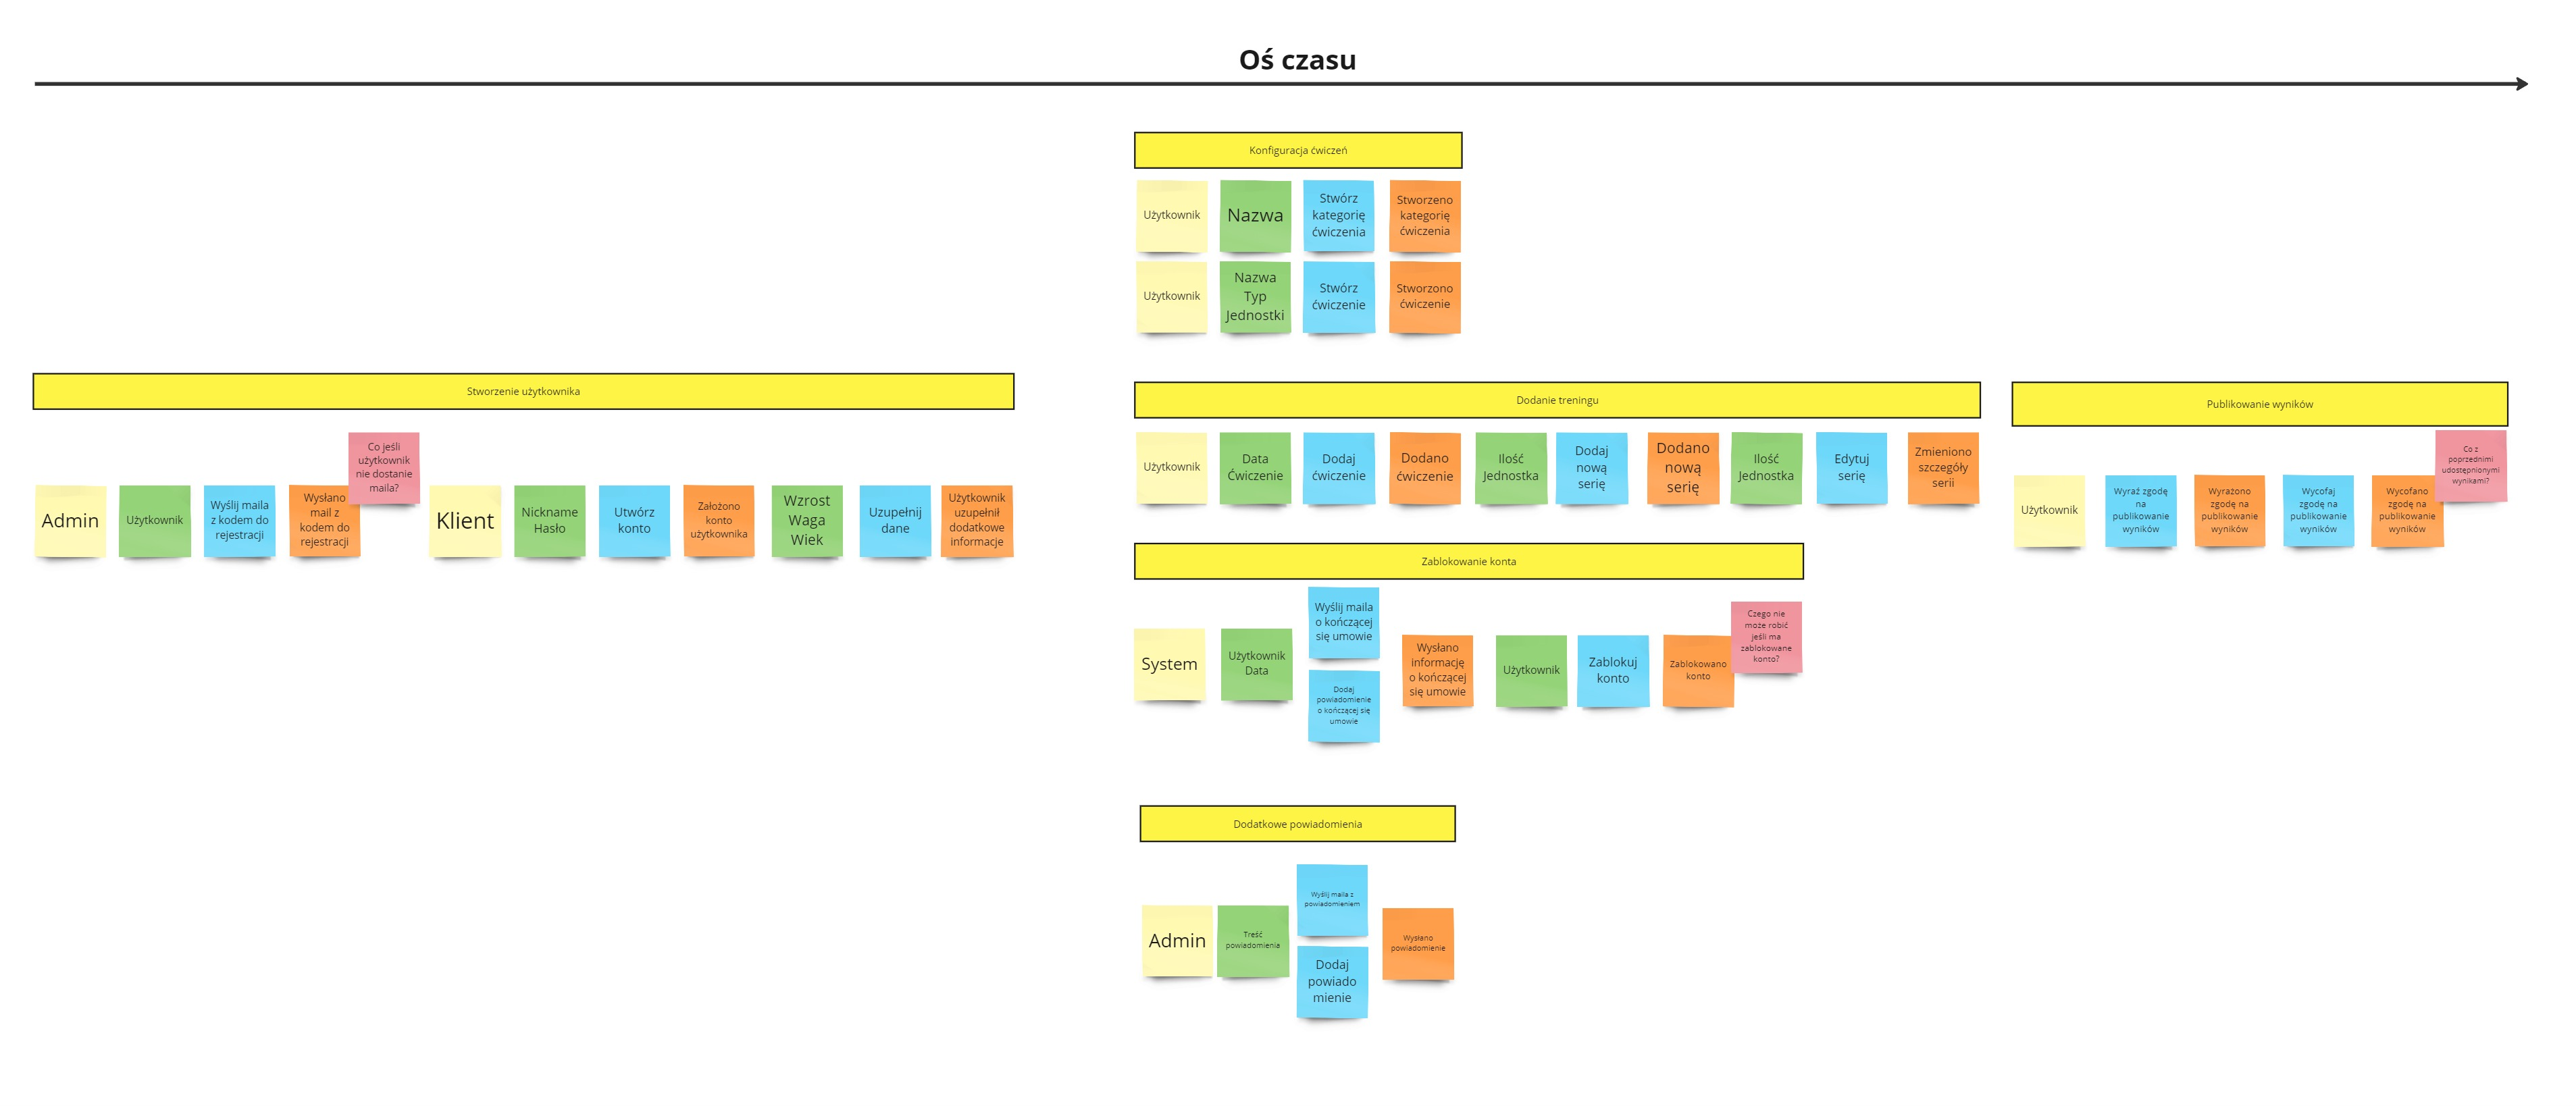
\includegraphics[width=0.9\linewidth]{ProcessLevel.jpg}
            \caption{Process level}
      \end{figure}


\end{document}